\chapter{绪论}
\section{引言}\label{section 1-1}

随着国民经济和社会的发展,以及人民对美好生活的追求,汽车已成为人们日常生活不可或缺的交通工具之一。
据统计,2021年底,全国民用汽车保有量高达30151万辆\cite{gou2022zhong}。
然而,汽车数量的急剧增长也给人类社会和自然环境带来了许多挑战。
根据世界卫生组织的数据,全球每年约有130万人因道路交通事故死亡,另外约有2000至5000万人因事故受到如致残等非致命伤害\cite{shi2022dao}。
同时,日益严峻的城市交通拥堵问题也给经济发展造成了巨大损失。
此外,汽车也是空气污染物排放的主要贡献者之一,仅在2021年,全国汽车污染物排放总量就超过1401.9万吨\cite{shen2022zhong}。
然而,随着传感技术、通讯方式和计算模式的发展,传统汽车正在向智能化、网联化和协同化方向迅速发展。
以智能网联汽车为抓手,车联网(Vehicle-to-Everything,简称V2X)驱动的智慧交通系统(Intelligent Transportation System,简称ITS)正致力于实现更加安全、高效和可持续发展的下一代交通运输。

近年来,车联网及其推动的智能网联汽车和智慧交通系统已成为我国的重要战略。
2019年9月,国务院发布了《交通强国建设纲要》,提出要加强智能网联汽车的研发,通过新基建形成自主可控的车联网核心技术与生态产业链 \cite{zhong2019jiao}。
2020年2月,国家发改委等11个部委联合发布了《智能汽车创新发展战略》,明确指出发展智能网联汽车对我国的重要战略意义,并将突破关键核心技术作为首要战略任务 \cite{guo2020zi}。
2022年8月,科技部发文支持建设包括智能港口、智能矿山和自动驾驶在内的十个新一代智能示范应用场景\cite{ke2022ke}。
与此同时,车联网商业化和相关基础设施的应用部署也是业界关注的热点领域。
2019年7月,华为发布了业界首款第五代移动通信技术(5th Generation Mobile Communication Technology,简称5G)车载通信模组MH5000,并与一汽、上汽、广汽等18家车企共同成立“5G汽车生态圈”,加速5G技术在汽车产业的商业进程,打造智能网联的5G汽车。
2020年10月,超过100家相关企业,包括传统汽车制造商、芯片模组与硬件制造商、地图与定位服务提供商在内,于中国上海开展了蜂窝车联网(Cellular-Vehicle-to-Everything,简称C-V2X)“新四跨”(跨芯片模组、跨终端、跨整车和跨安全平台)应用示范活动。
截至2023年2月,已有十几家车企推出了C-V2X量产车型,其中包括一汽、上汽、通用、上汽奥迪、广汽、长安福特、长城、比亚迪和蔚来等。

在学术研究方面,国内外众多一流高校与科研院所围绕车联网、车路协同、无人驾驶、智慧交通系统等领域展开了深入探索与研究。
在国内,由清华大学、长安大学与中国移动牵头成立了“车联网与智能汽车测试技术”创新联盟,联合推动车联网与智能汽车关键技术的研究与开发。
北京理工大学张军院士团队聚焦于“天空地网络”协同应用的智慧交通系统,通过多媒体站、车载导航、多媒体通道整合信息,实现“人、车、路”三者结合,取得了系列关键技术的创新与突破。
清华大学智能车路协同与自动驾驶研究中心张毅教授团队以车路协同环境为基础平台,重点研究了复杂混合交通群体智能决策机理与协同控制理论,以攻克车辆群体智能协同控制关键技术。
中科院复杂系统管理与控制国家重点实验室王飞跃教授团队在智能交通的信息物理融合方面取得了重要突破。
长安大学赵样模教授团队围绕高速公路场景下的智能车路协同体系架构以及相关运行安全性与适应性评估技术展开了深入的研究,并联合多家优势单位共同在京沪高速开展了应用示范。
西安电子科技大学综合业务网理论与关键技术国家重点实验室毛国强教授团队在车联网的高效数据分发、实时感知、智能应用等方面均取得了具有国际影响力的科研成果。
无线移动通信国家重点实验室陈山枝教授团队致力于5G-V2X 标准的制定及关键技术的研究,极大推动了车联网产业化进展。
在国际上,加拿大滑铁卢大学Sherman Shen教授的团队在车联网安全、车辆间通信、车路协同、资源优化、智慧交通系统和车辆协同智能等多个领域取得了重要的研究突破。
加拿大英属哥伦比亚大学Victor C.M Leung教授的团队专注于车联网边缘缓存、信息安全和无线传输协议等领域的研究,并取得了重要的科研成果。
瑞典奥斯陆大学Yan Zhang教授的团队在车联网端边云协同、自适应任务协作、负载均衡和隐私保护等方面做出了突出的贡献。
日本东北大学Nei Kato教授的团队在车载自组织网络的安全、拓扑控制和路由协议等方面进行了全面深入的研究,并获得了系列原创性研究成果。

“信息物理系统(Cyber-Physical System,简称CPS)”一词是由美国国家科学基金会的Helen Gill约于2006年提出的\cite{lee2016introduction}。
随着多年的研究和发展,自从Li等人于2011年首次将CPS应用于车联网中,车载信息物理融合系统(Vehicular Cyber-Physical System,简称VCPS)\cite{li2011human}已成为国内外学术界热门研究领域之一。
VCPS是一个集智能网联汽车、车联网、边缘计算、云计算等多种技术于一体的系统,利用智能网联汽车的多模态感知能力、V2X通信技术以及边缘端和云端的存储和计算资源,形成一个感知-传输-计算一体化的综合系统。
此外,它还利用车辆的多源感知物理信息,在边缘端或云端构建信息层面的逻辑视图,以支持智慧交通系统中多样化的应用。
然而,由于车联网具有异构高动态、物理环境分布式时变、节点资源动态异构、应用需求多元、真实环境复杂等特点,因此实现面向异构车联网的车载信息物理融合系统仍然面临巨大挑战。
本文将结合车联网特点和智慧交通系统的多样化应用需求,在系统架构、指标设计、算法策略和系统实现方面进行理论和技术上的综合创新,提炼出异构车联网融合、逻辑视图质量评估、协同资源优化、VCPS质量-开销均衡以及复杂真实环境下系统实现等关键问题,并提出相应的解决方案,以实现面向异构车联网的车载信息物理融合系统。

\section{研究背景}\label{section 1-2}

本节将首先介绍车联网的相关概念,随后以碰撞预警系统为例,介绍车载信息物理融合系统,并进一步分析其中所面临的挑战。

车联网是物联网(Internet of Things,简称IoT)技术在汽车领域的一种应用形式。
具体而言,车联网是指多种通讯方式的融合,包括车辆间通讯(Vehicle-to-Vehicle,简称V2V)、车辆与行人通讯(Vehicle-to-Pedestrian,简称V2P)、车辆与基础设施通讯(Vehicle-to-Infrastructure,简称V2I)以及车辆与云端通讯(Vehicle-to-Cloud,简称V2C)。
车联网利用实时数据分发,实现人、车、路等交通要素的协同配合,最终实现“聪明的车、智慧的路、协同的云”。
进一步地,车联网还能配合基于单车智能的自动驾驶技术发展,通过车联网通信协助自动驾驶判断隐藏危险,提升道路安全。
随着我国车联网产业在政策规划、标准体系建设、关键技术研发、应用示范和基础设施建设等多方面的稳步发展,车联网的内涵和外延也在不断发展演进。
依托快速落地的新型基础设施建设,车联网不仅广泛服务于智能网联汽车的辅助驾驶、自动驾驶等不同应用,而且拓展服务于智慧矿山、智慧港口等企业生产环节以及智慧交通、智慧城市等社会治理领域 \cite{zhong2021che}。

\begin{table}[h]
\centering
\bicaption{C-V2X和IEEE 802.11p技术对比}{Technical comparisons of C-V2X and IEEE 802.11p}
\label{table 1_1}
\resizebox{\columnwidth}{!}{%
\begin{tabular}{@{}ccccc@{}}
\toprule
\begin{tabular}[c]{@{}c@{}}C-V2X\\ 技术优势\end{tabular} &
 \begin{tabular}[c]{@{}c@{}}具体技术\\ 或性能\end{tabular} &
IEEE 802.11p &
\begin{tabular}[c]{@{}c@{}}LTE-V2X\\ (3GPP R14/R15)\end{tabular} &
\begin{tabular}[c]{@{}c@{}}NR-V2X\\ (3GPP R16)\end{tabular} \\ \midrule
低时延 &
  时延 &
  不确定时延 &
  \begin{tabular}[c]{@{}c@{}}R14: 20ms\\ R15: 10ms\end{tabular} &
  3ms \\ 
\begin{tabular}[c]{@{}c@{}}低时延/\\ 高可靠\end{tabular} &
  \begin{tabular}[c]{@{}c@{}}资源分配\\ 机制\end{tabular} &
  CSMA/CA &
  \begin{tabular}[c]{@{}c@{}}支持感知+半持续\\ 调度和动态调度\end{tabular} &
  \begin{tabular}[c]{@{}c@{}}支持感知+半持续\\ 调度和动态调度\end{tabular} \\ 
\multirow{3}{*}[3.4ex]{高可靠} &
  可靠性 &
  不保证可靠性 &
  \begin{tabular}[c]{@{}c@{}}R14: \textgreater{}90\%\\ R15: \textgreater{}95\%\end{tabular} &
  支持99.999\% \\  
 &
  信道编码 &
  卷积码 &
  Turbo &
  LDPC \\ 
 &
  重传机制 &
  不支持 &
  \begin{tabular}[c]{@{}c@{}}支持HARQ,\\ 固定2次传输\end{tabular} &
  \begin{tabular}[c]{@{}c@{}}支持HARQ,\\ 传输次数灵活,\\ 最大支持32次传输\end{tabular} \\ 
\multirow{2}{*}[0ex]{\begin{tabular}[c]{@{}c@{}}更远传输\\ 范围\end{tabular}} &
  通信范围/m &
  100 &
  \begin{tabular}[c]{@{}c@{}}R14: 320\\ R15: 500\end{tabular} &
  1000 \\  
 &
  波形 &
  OFDM &
  \begin{tabular}[c]{@{}c@{}}单载波频分复用\\ (SC-FDM)\end{tabular} &
  循环前缀(CP)-OFDM \\ 
\multirow{2}{*}[1.5ex]{\begin{tabular}[c]{@{}c@{}}更高传输\\ 速率\end{tabular}} &
  \begin{tabular}[c]{@{}c@{}}数据传输\\ 速率\end{tabular} &
  典型6Mbit/s &
  \begin{tabular}[c]{@{}c@{}}R14: 约30Mbit/s\\ R15: 约300Mbit/s\end{tabular} &
  \begin{tabular}[c]{@{}c@{}}与带宽有关,40MHz\\ 时R16单载波2层数据\\ 传输支持约400Mbit/s,\\ 多载波情况下更高\end{tabular} \\ 
 &
  调制方式 &
  64QAM &
  64QAM &
  256QAM \\ \bottomrule
\end{tabular}%
}
\end{table}

在车联网通信标准方面,电气和电子工程师协会(Institute of Electrical and Electronics Engineers,简称 IEEE)于2003年提出了DSRC,它是一种用于车联网通信的专用短程通信技术。
2010年,IEEE正式发布了名为车载环境无线接入(Wireless Access in Vehicular Environments,简称 WAVE)的协议栈,其中包括IEEE 802.11p、IEEE 1609.1/.2/.3/.4协议族和SAE J2735消息集字典\cite{wu2013vehicular}。
DSRC使用5.9GHz频段中的75MHz频谱资源,被划分为1个控制信道和6个服务信道,并可通过支持DSRC技术的OBU和RSU实现V2V和V2I通信。
同时,随着基于蜂窝的移动通信技术的快速发展,长期演进车辆通信(Long-Term Evolution-Vehicle, 简称LTE-V)已经形成了一个较为完善的技术标准体系和产业链 \cite{chen2016lte}。
此外,作为中国5G技术创新主要平台的 IMT-2020(5G)推进组于2017年成立了C-V2X工作组,以加速向基于5G的V2X通信演进。
国际标准组织第三代合作伙伴计划(3rd Generation Partnership Project,简称 3GPP)于2020年完成了Rel-16版本的5G NR-V2X标准,并在Rel-17版本中进一步优化了功率控制、资源调度等相关技术。
我国LTE-V2X产业已经蓬勃发展,与DSRC的技术路线之争取得重大进展。
我国已建成基于LTE-V2X技术的完备产业链,芯片、模组、OBU、RSU等都已成熟且经过了“三跨”“四跨”“新四跨”以及大规模测试,满足了商用部署条件。
5G 汽车协会(5G Automotive Association,简称 5GAA)、下一代移动通信网络(Next Generation Mobile Network, 简称 NGMN)联盟以及5G Americas对IEEE 802.11p和C-V2X进行了技术对比,表明C-V2X在低时延、高可靠性、资源利用率等方面具有技术优势。具体对比见表\ref{table 1_1} \cite{cheng2021feng}。

\begin{figure}[h] % use float package if you want it here
	\centering
	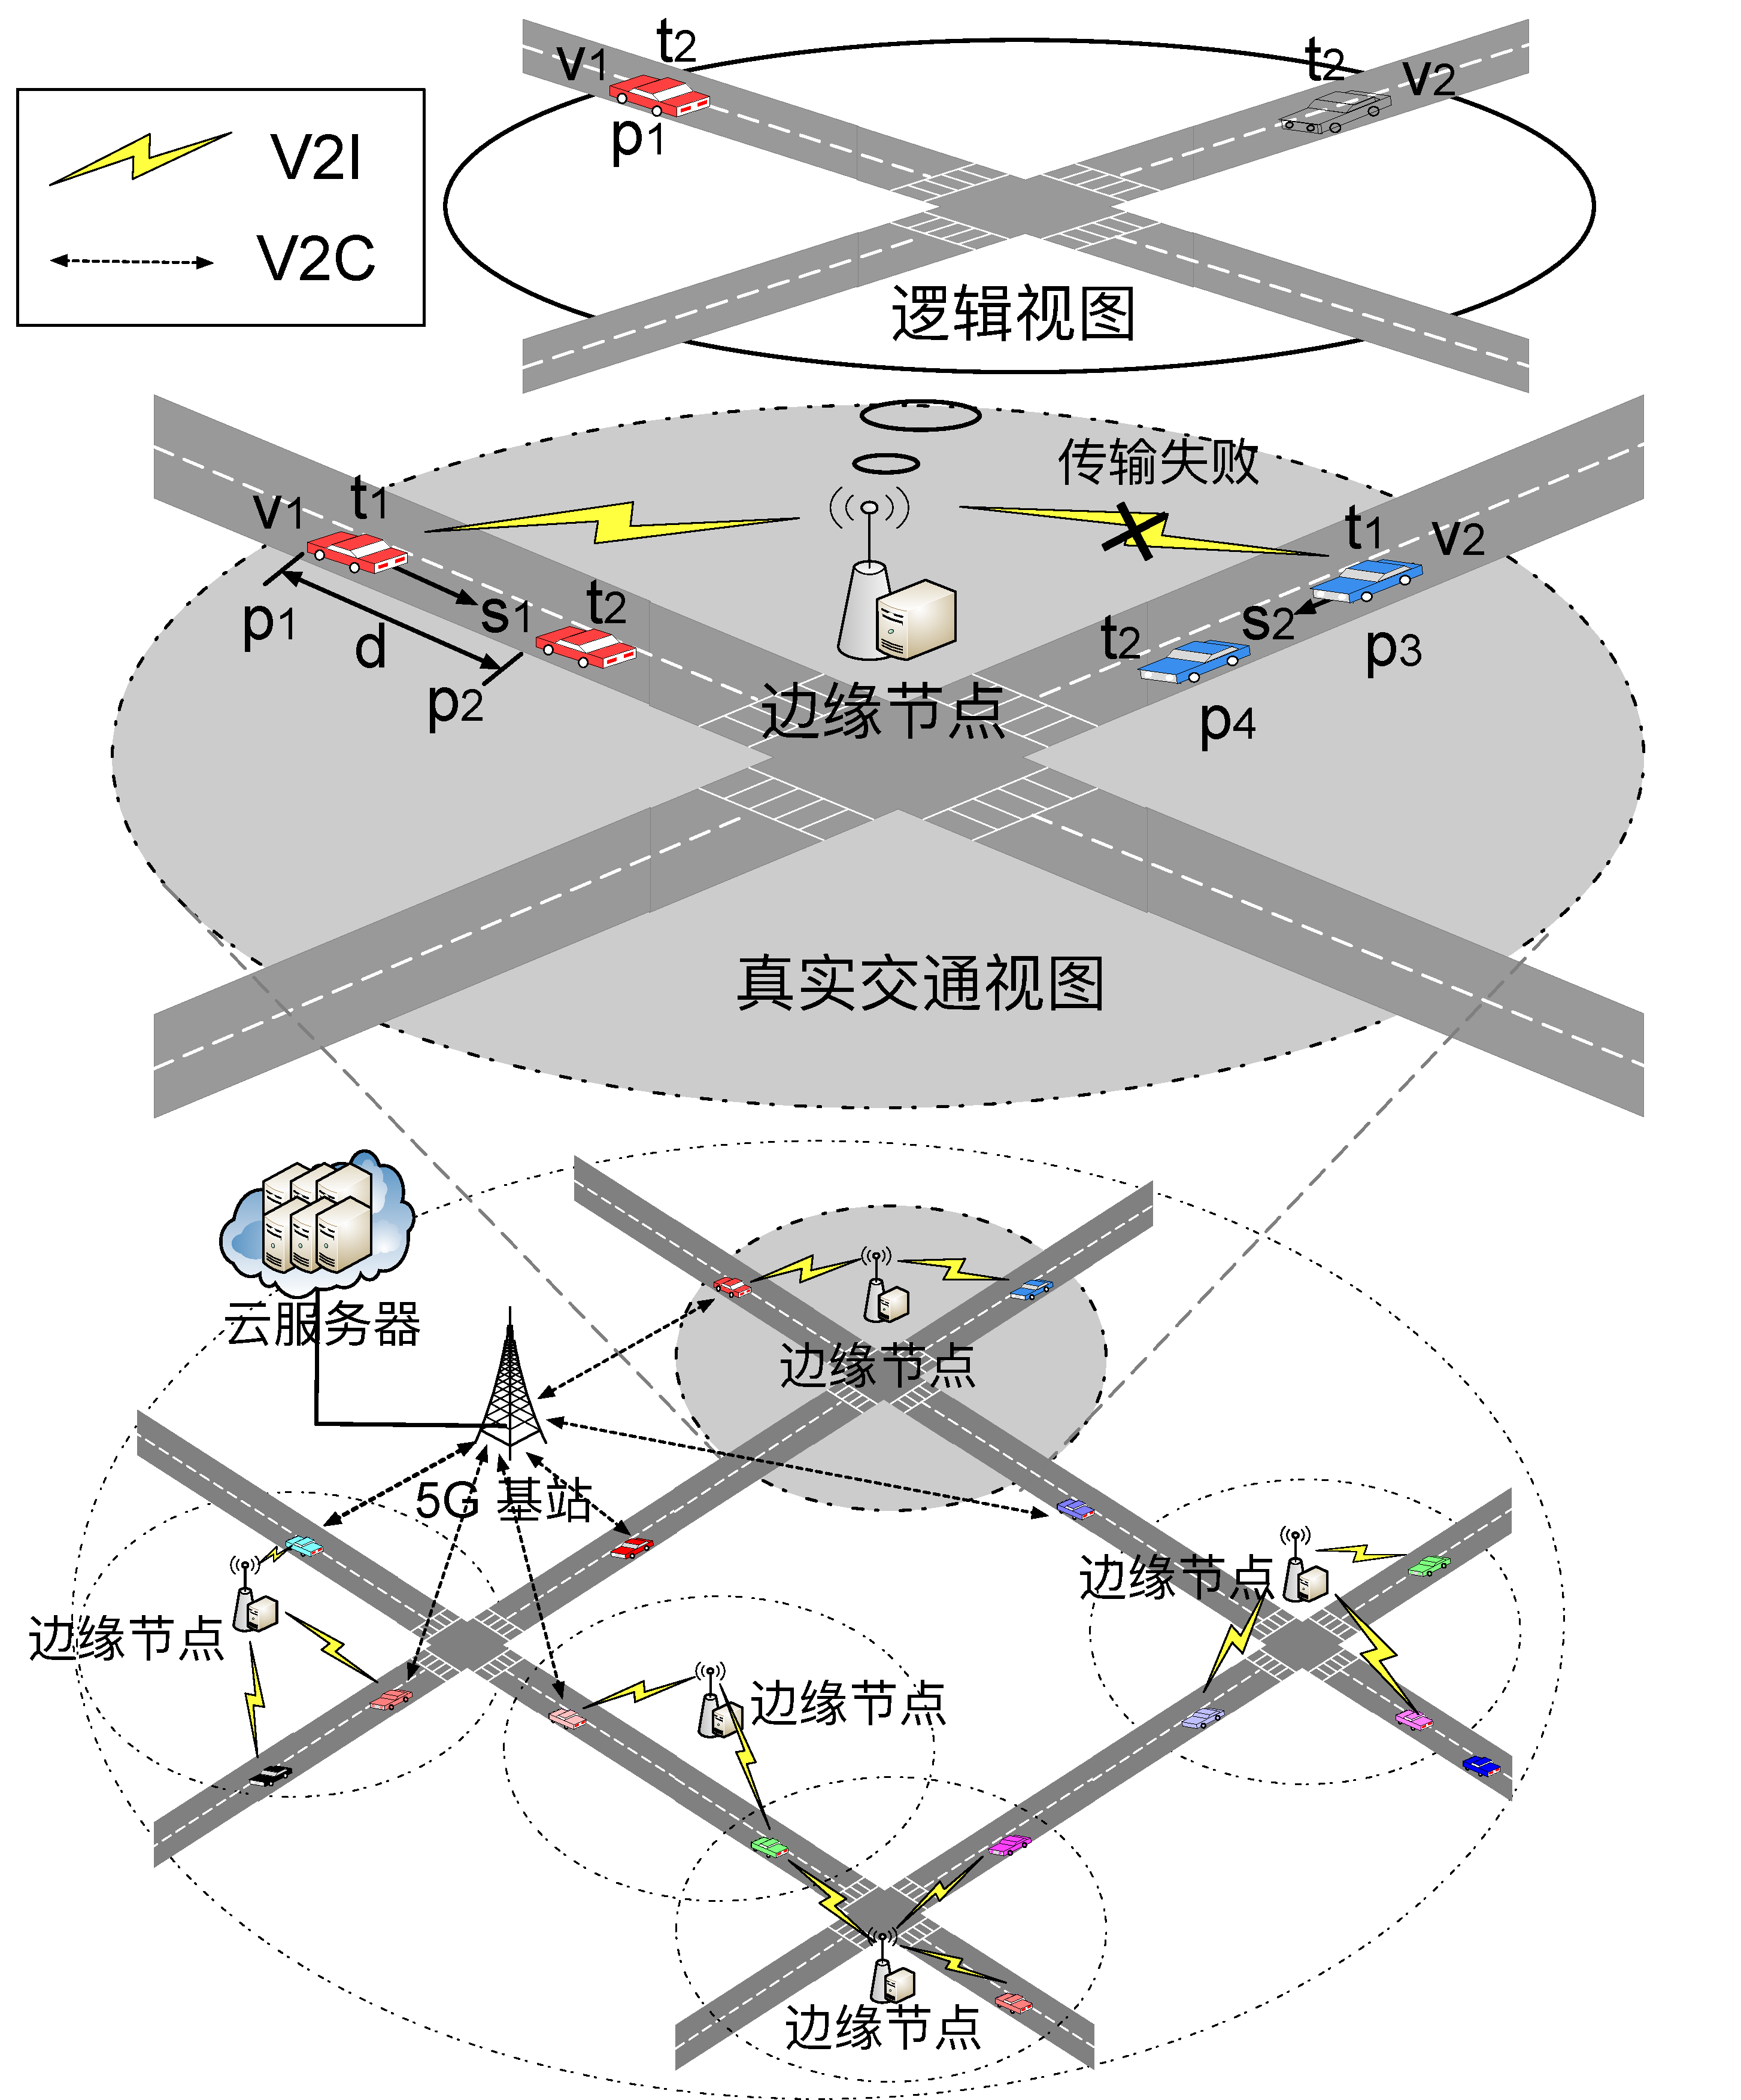
\includegraphics[width=0.9\columnwidth]{Fig1-1-example.pdf}
	\bicaption{基于逻辑视图的碰撞预警系统}{Collision warning system based on the logical view}
	\label{fig 1-1}
\end{figure}

本章节以碰撞预警系统为例,阐述车联网中车载信息物理融合系统构建过程及其重要性。
首先,碰撞预警系统作为智慧交通系统中典型安全应用,对于预防交通事故具有重要意义。
如图 \ref{fig 1-1} 所示,具有短无线电覆盖范围的通信基础设施(如RSU、5G小基站)可被作为边缘节点,因为它们在物理位置上更接近车辆并具有一定的计算能力。
另一方面,具有广泛覆盖范围的通信基础设施(如 5G 蜂窝网络基站)可被视为云节点。
车辆可通过 V2C 和 V2I 通信分别与云节点和沿路安装的边缘节点进行通信。
其中,云节点被认为具有无限的计算能力,但如果其覆盖范围内的所有车辆都在并发地传输数据,它可能会遭受严重的带宽竞争。 
考虑到两辆汽车(即图中 $v_1$ 和 $v_2$ )正在接近一个没有交通信号灯的十字路口,那么很可能会发生碰撞,特别是在互相看不见对方的情况下。
在该系统中,车辆定期通过 V2I 通信将实时状态上传至边缘节点,包括全球定位系统(Global Positioning System,简称 GPS)坐标、速度、加速度、方向等。
边缘节点处理车辆的传感数据,并构建出实时反映车辆状态的逻辑视图以支持基于车辆轨迹预测的碰撞预警服务。
然而,不可避免的是传感数据是不准确的,例如,由于卫星时钟偏差、大气延迟和广播星历错误等原因,获得的 GPS 坐标是不准确的 \cite{liu2013improving}。
此外,无线通信中的数据包丢失使得边缘节点估计移动车辆的实时位置变得更加困难。

如上分析,尽管边缘计算新范式比传统的集中式云计算减少了通信延迟,但由于不可避免及不可忽视的诸如传感器错误、传输延迟和数据包丢失等问题,碰撞预警系统仍然会受到车辆信息不准确的影响。
图 \ref{fig 1-1} 中的放大部分显示了在边缘节点构建的逻辑视图与真实交通视图相比,车辆位置不准确的例子。
具体来说,假设车辆$v_1$在时间$t_1$的位置为以$p_1$并以$s_1 =$ 40 km/h 的速度接近十字路口。
同时,车辆$v_2$在时间$t_1$位于$p_3$并以$s_2=$ 25 km/h的速度接近同一路口。
车辆$v_1$和$v_2$在时间$t_1$同时向边缘节点发送它们的状态,然而,包含车辆$v_2$状态的数据包在V2I通信中丢失。
边缘节点在时间$t_2$接收车辆状态信息,并形成一个关于每个车辆位置的逻辑视图,如图\ref{fig 1-1}顶部所示。
假设数据大小为 500 kB,这对于典型的ITS应用来说是足够的\cite{liu2013improving}。
典型的车联网通信技术DSRC支持3$\sim$27 Mb/s的数据速率,其中3 Mb/s 被推荐用于传输安全关键信息\cite{kenney2011dedicated}。
因此,上传车辆状态的时间约为500 * 8 kb / 3 $\approx$ 1.3 s,即${t_2} - {t_1} \approx 1.3$ s。
车辆$v_1$在时间$t_2$位于$p_1$,而$v_2$在边缘节点的逻辑视图中不存在。
然而如现实交通视图所示,车辆$v_1$和$v_2$的现实位置分别为$p_2$和$p_4$。
边缘节点的逻辑车辆视图和现实交通视图之间的车辆$v_1$位置的距离误差约为40 * 1000 / 3600 m/s * 1.3 $\approx$ 14 m,换言之,$d \approx$ 14 m。
通过上述例子,显然,如何在异构车联网中实现信息物理融合即构建一个实时准确的视图以支持不同的智慧交通系统应用是当前迫切需要且极具挑战的问题。

\section{国内外研究现状}\label{section 1-3}
% VCPS 论文分类,优先级top

面向异构车联网的车载信息物理融合系统是实现各类智慧交通系统应用的基础,其已成为国内外学术界的研究热点之一。
本节对国内外相关研究工作进行了梳理和总结,现从以下几个方面进行详细阐述。

\subsection{车联网服务架构与应用研究}

对于车联网中的服务架构,研究人员在研究基于软件定义网络(Software Defined Network,简称SDN)和边缘计算的范式方面付出了巨大努力。
He等人\cite{he2016sdvn}提出了一个基于SDN的架构,以实现异构车辆通信环境中的快速网络创新。
Huang等人\cite{huang2017exploring}提出了用于提供服务的5G支持的软件定义车辆网络(Software Defined Vehicular Network, SDVN)。
Liu等人\cite{liu2016cooperative}提出了一种SDVN中的调度算法,用于通过混合V2I/V2V通信进行合作数据传播。
Dai等人\cite{dai2018cooperative}提出了在异构车辆网络中基于SDN的时间约束的时间信息服务的调度。
Luo等人\cite{luo2018sdnmac}提出了一个基于SDN的介质访问控制(MAC)协议,以提高动态车辆网络环境中的通信性能。
Liu等人\cite{liu2018coding}提出了一个基于SDN的服务架构,并结合车辆缓存和网络编码来提高带宽效率。
Stojmenovic和Wen\cite{stojmenovic2014the}首次提出将雾计算融入SDVN。
Zhang等人\cite{zhang2017cooperative}提出了一个用于物联网大数据处理的合作式雾计算架构。
Hou等人\cite{hou2016vehicular}提出了一个车辆雾计算(VFC)架构,在这个架构中,车辆被视为移动基础设施,它们各自的资源被聚合起来,以获得更好的通信和计算服务。
Huang等人\cite{huang2017vehicular}提供了一个雾辅助交通控制系统的案例研究,并讨论了基于VFC服务的潜在好处、安全问题和取证挑战。
Ning等人\cite{ning2019vehicular}提出了一个具有云、小云和雾层的VFC架构,它被应用于智能城市的分布式实时交通管理。

研究人员对面向车载边缘计算的车载应用做出了巨大的努力。
Liu等人\cite{liu2021fog}研究了终端-边缘-云合作架构中的合作数据传播问题。提出了一种基于Clique的算法来联合安排数据编码和传播。
Dai等人\cite{dai2021edge}设计了一个基于自适应比特率的多媒体流的VEC架构,其中边缘缓存和传输服务被提供给以不同质量等级编码的文件块。
Zhang等人\cite{zhang2022digital}提出了一种社会感知的车辆边缘缓存技术,该技术基于用户偏好的相似性和服务的可用性,动态地协调边缘节点和智能车辆的缓存能力。
Liu等人\cite{liu2020adaptive}提出了一个两层的VEC架构,利用云、静态边缘节点和移动边缘节点来处理时间紧迫的任务。
Liu等人\cite{liu2018coding}提出了一种记忆算法,利用车辆缓存和网络编码之间的协同效应,提高VEC中数据广播的带宽效率。

关于车辆网络中的数据传播、信息缓存和任务卸载的研究已经很多了。
Liu等人\cite{liu2021fog}考虑了车辆终端-云结构中的合作数据传播问题,并提出了一个基于clique搜索的调度方案,以实现合作数据编码和传播。
Singh等人\cite{singh2020intent}提出了一个基于意图的网络控制框架,其中一个神经网络被用来训练流表,并实现了智能数据传播。
Dai等人\cite{dai2020deep}提出了一个支持区块链的分布式信息缓存框架,它整合了DRL和许可区块链,实现了智能和安全的信息缓存。
Su等人\cite{su2018an}开发了一种基于分析车辆内容请求特征的动态信息缓存方案。
Shang等人\cite{shang2021deep}研究了节能的任务卸载,并开发了一种基于深度学习的算法来最小化能耗。
Liao等人\cite{liao2021learning}提出了一种空地一体的VEC的任务卸载策略,使车辆能够学习具有多维意图意识的长期策略。
这些研究主要集中在车辆网络中的数据传播、信息缓存和任务卸载的调度算法上。然而,他们都没有研究VCPS中合作感知和异质信息融合的协同效应。


\subsection{车载信息物理融合系统评估指标研究}

研究人员在VCPS的预测、调度和控制技术方面付出了巨大努力。
Zhang等人\cite{zhang2019a}提出了一种混合速度-轮廓预测方法,该方法将交通流状态与个人驾驶行为相结合。
Zhang等人\cite{zhang2020data}在变道行为预测模型和加速预测模型的基础上预测了车辆状态。
Li等人\cite{li2020cyber}考虑了车辆的流动性,并开发了一个基于物理比率-K干扰模型的广播方案以确保通信的可靠性。
Lian等人\cite{lian2021cyber}提出了一种基于既定地图模型的路径规划的调度方法,以优化路径利用效率。
Dai等人\cite{dai2016a}提出了一种自主交叉口控制机制,以确定车辆通过交叉口的优先权。
Hu等人\cite{hu2017cyber}提出了一种燃油最优控制器,根据领先车辆的状态优化车辆速度和无级变速箱齿轮比。
Lv等人\cite{lv2018driving}提出了一种自适应算法,用于控制三种典型驾驶方式下不同协议选择的车辆加速。
这些研究集中在支持VCPS的不同技术上,如轨迹预测、路径调度和车辆控制,这促进了各种ITS应用的实施。然而,这些研究是基于对车辆网络中物理元素建模的质量信息的可用性的假设,没有对逻辑视图的质量进行定量分析。

一些研究对VCPS中的信息质量进行了评估。
Liu等人\cite{liu2014temporal}提出了一种用于VCPS中时间性数据传播的调度算法,该算法在实时数据传播和及时信息感知之间取得了平衡。
Dai等人\cite{dai2019temporal}提出了一种进化的多目标算法,以提高信息质量,改善数据交付率。
Liu等人\cite{liu2014scheduling}提出了两种在线算法,通过分析传播特性来安排不同一致性要求下的时间性数据传播。
Rager等人\cite{rager2017scalability}开发了一个框架,通过对随机数据负载进行建模来提高信息质量,以捕捉真实网络的随机性。
Yoon等人\cite{yoon2021performance}提出了一个统一的合作感知框架,考虑到车辆网络中的通信损耗和车辆的随机运动,以获得车辆的精确运动状态。
这些研究集中在VCPS中数据及时性、准确性或一致性方面的信息质量评估。然而,现有的研究只考虑了同质数据项层面的质量测量,这在考虑应用层面时可能是不够的,因为所需的逻辑视图是通过融合异质信息构建的。

\subsection{车联网资源分配与任务卸载研究}

一些研究人员已经在车辆网络中利用非正交多址接入(Non-Orthogonal Multiple Access,简称 NOMA)技术来进一步提高带宽效率。
Patel等人\cite{patel2021performance}评估了基于NOMA的车辆网络的通信容量,数值结果显示,NOMA比传统的OMA高出约20\%。
Zhang等人\cite{zhang2021centralized}利用基于图的匹配方法和通过非合作博弈的分布式功率控制,为NOMA集成的车辆网络开发了一个集中的两阶段资源分配策略。
Zhu等人\cite{zhu2021decentralized}提出了一种考虑随机任务到达和信道波动的最优功率分配策略,以最大化长期的功率消耗和延迟。
Liu等人\cite{liu2019energy}提出了在基于NOMA的自动驾驶汽车网络中分配功率的乘法技术的替代方向算法。
尽管如此,这些研究主要是基于单边缘节点的情况,而不同边缘节点之间的干扰无法处理。

一些研究专注于VEC中的任务卸载或资源分配。
Liu等人\cite{liu2021rtds}通过评估VEC中的移动性感知的通信模型、资源感知的计算模型和截止日期感知的奖励模型,提出了一种多周期任务卸载的实时分布式方法。
Liu等人\cite{liu2022a}提出了一种结合乘法交替方向法和粒子群优化的任务卸载算法,以最小化执行延迟、能源消耗和支付成本的加权和。
Chen等人\cite{chen2020robust}提出了一种带有故障恢复功能的计算卸载方法,以减少能源使用并缩短应用完成时间。
Liu等人\cite{liu2014temporal}通过考虑数据传播的时间限制和数据项的新鲜度,提出了一种用于实时数据传播的启发式调度算法。
Liu等人\cite{liu2016cooperative}开发了一种用于混合车辆通信环境下合作数据传播的贪婪方法。
然而,他们都没有研究实时任务卸载和通信/计算资源分配的协同效应。

一些研究考虑了VEC的联合通信和计算资源分配。
Cui等人\cite{cui2021reinforcement}提出了一种多目标的强化学习方法,通过结合通信和计算资源分配来减少系统延迟。
Han等人\cite{han2020reliability}通过动态编程方法提出了面向耦合的车辆通信和计算的可靠性计算。
Xu等人\cite{xu2021socially}采用契约理论为每个潜在的内容供应商和内容请求者对分配通信和计算资源。
少数研究者研究了联合任务卸载和资源分配。
Dai等人\cite{dai2021asynchronous}提出了一个异步的深度强化学习,用于考虑异构服务器的数据驱动的任务卸载,如强大的车辆、VEC服务器和云。
Dai等人 \cite{dai2022a}开发了一种概率计算卸载方法,用于根据边缘节点的计算分配概率独立调度计算卸载。
然而,现有的研究不能应用于大规模的车辆网络,因为它们主要是基于集中式调度,具有较高的通信开销和调度复杂性。

\subsection{车联网中强化学习应用研究}

一些研究专注于在车辆网络中使用MADRL的任务卸载或资源分配\cite{althamary2019a}。
Alam等人\cite{alam2022multi}开发了一种基于DRL的多代理匈牙利算法(MADRLHA),用于VEC中的动态任务卸载,以保证延迟、能耗和支付费用的要求。
Zhang等人\cite{zhang2021adaptive}提出了一种用于边缘资源分配的MADDPG方法,以在严格的延迟约束下最小化车辆任务卸载成本。
Nie等人\cite{nie2021semi}提出了一种多代理联合强化学习(MAFRL)算法,在无人机(UAV)支持的VEC中联合优化资源分配、用户关联和功率控制。
博弈论和强化学习的结合最近引起了学术界的广泛关注。
Zheng等人\cite{zheng2022stackelberg}将基于行动者-评论家的强化学习的行为者和批评者之间的互动建模为具有领导者-追随者结构的两局一般和博弈。
Albaba等人\cite{albaba2021driver}将DQN和层次博弈论结合起来,对高速公路驾驶场景中的司机进行行为预测,其中k级推理被用来模拟人类司机的决策过程。
Rajeswaran等人\cite{rajeswaran2020a}开发了一个框架,将基于模型的强化学习作为政策参与者和模型参与者之间的Stackelberg博弈。
然而,这些解决方案都不能直接应用于车辆网络,用于联合实时任务卸载和异质资源分配。

一些研究侧重于通过使用DRL算法进行车辆传感和信息融合。
Zhao等人\cite{zhao2020social}设计了一个基于近似策略优化(PPO)的社会意识激励机制,以得出最佳的长期传感策略。
Dong等人\cite{dong2020spatio}提出了一种基于深度Q网络(DQN)的方法,以融合在当地下游环境中获得的信息,从而做出可靠的车道变更决策。
Mika等人\cite{mlika2022deep}提出了一个基于深度确定性策略梯度(DDPG)的解决方案,通过调度资源块和广播覆盖来最小化信息的年龄。
这些技术主要是针对车辆传感和信息融合提出的,使用单代理DRL算法,如DQN、DDPG和PPO。然而,这些算法不能直接应用于VCPS中的合作感知和异构信息融合,而且当考虑到多辆车时,这些算法并不适合。少数研究将多代理DRL应用于车辆网络的资源分配。
He等人\cite{he2021efficient}提出了一种多代理行动者-评论家(MAC)算法,为具有严格延迟要求和最小带宽消耗的车辆分配资源。
尽管如此,这些解决方案只考虑了车辆网络中一种类型的代理(即车辆或边缘节点)。

\section{研究目标与研究内容}\label{section 1-4}
\subsection{研究目标}

本文针对车联网异构环境、分布式时变物理环境、动态受限节点资源,以及多元智慧交通系统应用需求所带来的挑战,从服务架构设计、评估指标设计、协同资源分配、质量开销均衡以及原型系统实现五方面,对面向异构车联网的车载信息物理融合系统展开研究。
基于上述描述,本文的研究目标包括如下:

\circled{1} 实现面向异构车联网的融合服务架构,为车载信息物理融合系统提供服务架构基础。首先,结合软件定义网络、网络功能虚拟化(Network Functions Virtualization,缩写NFV)与网络切片等关键思想,提出基于 SDN 的分层服务架构,以支持系统面向大规模数据服务的灵活性、可靠性及可扩展性。其次,考虑控制层、虚拟化层、数据层面临的挑战,设计跨层协议栈。最后,基于边缘计算范式,实现集中控制与分布式调度的有机结合,进一步提高系统的可靠性与可扩展性。

\circled{2} 实现面向车联网时变物理信息的分布式感知与边缘视图构建,为车载信息物理融合系统提供评估指标。首先,面向车载边缘计算环境,提出基于多类M/G/1的信息感知排队模型。进一步,针对边缘视图对于感知信息的时效性、完整性以及一致性需求,设计VCPS评估指标,即Age of Viev,实现车辆协同信息感知与边缘侧的异质信息融合。最后,建立边缘视图质量评估模型,并基于多智能体强化学习,提出针对边缘视图质量的物理感知优化策略,实现高效实时的边缘视图构建。

\circled{3} 实现面向动态异构车联网节点资源的异构资源协同优化,为车载信息物理融合系统提供技术支撑。首先,面向NOMA车联网的车载边缘计算环境,提出 V2I 传输与任务卸载模型。进一步,建立协同资源优化博弈模型,并分解为资源调度与任务卸载两个子问题。最后,一方面,针对资源调度子问题,基于凸优化理论提出资源分配策略,另一方面,针对任务卸载子问题,基于多智能体 D4PG 算法提出资源分配策略,实现基于边缘协同的异构资源利用效率最大化。

\circled{4} 实现面向多元智慧交通系统应用需求的 VCPS 质量-开销均衡优化,为车载信息物理融合系统提供理论保障。首先,面向多元智慧交通系统应用需求,针对车联网中不同交通要素,建立相应的数字孪生模型。进一步,综合考虑数字孪生模型的差异性数据需求,建立车载信息物理融合系统的质量与开销模型。最后,基于多目标强化学习,提出车载信息物理融合系统的质量与开销均衡策略,实现质量-开销均衡的车载信息物理融合。

\circled{5} 建立软件仿真环境、硬件在环测试平台,以及小规模真实车联网边缘智能场景,综合验证所提模型、机制与算法的可行性与有效性。首先,基于真实车辆轨迹与地图信息搭建交通仿真平台。其次,搭建基于真实OBU(端)、RSU(边)的通信与计算环境,及基于LTE/5G 的远程服务器通信与计算平台(云),实现硬件在环性能验证。最后,基于真实车联网环境,实现基于车载信息物理融合的超视距碰撞预警原型系统,进一步验证所提计算模型与优化策略。

\subsection{研究内容}
% 研究内容框架图

本文致力于研究面向异构车联网的车载信息物理融合系统,主要研究内容及关系如图 \ref{fig 1-2} 所示。
首先,面向高动态异构车联网,融合不同的计算范式与服务架构是实现车载信息物理融合的服务架构基础。
因此,本文将首先研究如何设计基于软件定义网络和边缘计算的融合车联网架构。
其次,面向分布式时变物理环境,有效的数据获取与建模评估是驱动车载信息物理融合的核心。
因此,本文将研究如何评估并提高车载边缘侧所构建的逻辑视图质量。
再次,面对动态异构节点资源,高效的任务调度与资源分配是进一步提升智慧交通系统服务质量的关键。
因此,本文将进一步研究如何实现节点间协同,提高异构资源利用效率。
面向多元智慧交通系统应用需求,满足差异性的系统质量与系统开销是驱动车载信息物理融合的另一关键。
因此,本文将更进一步研究VCPS质量/开销模型及其优化策略。
最后,面向复杂的真实车联网环境,基于车载信息物理融合系统进行有效设计并实现具体系统原型是具有挑战的。
因此,本文将深入研究基于车载信息物理融合系统的超视距碰撞预警原型系统设计与实现。本文具体研究内容如下所述。

\begin{figure}[h] % use float package if you want it here
	\centering
	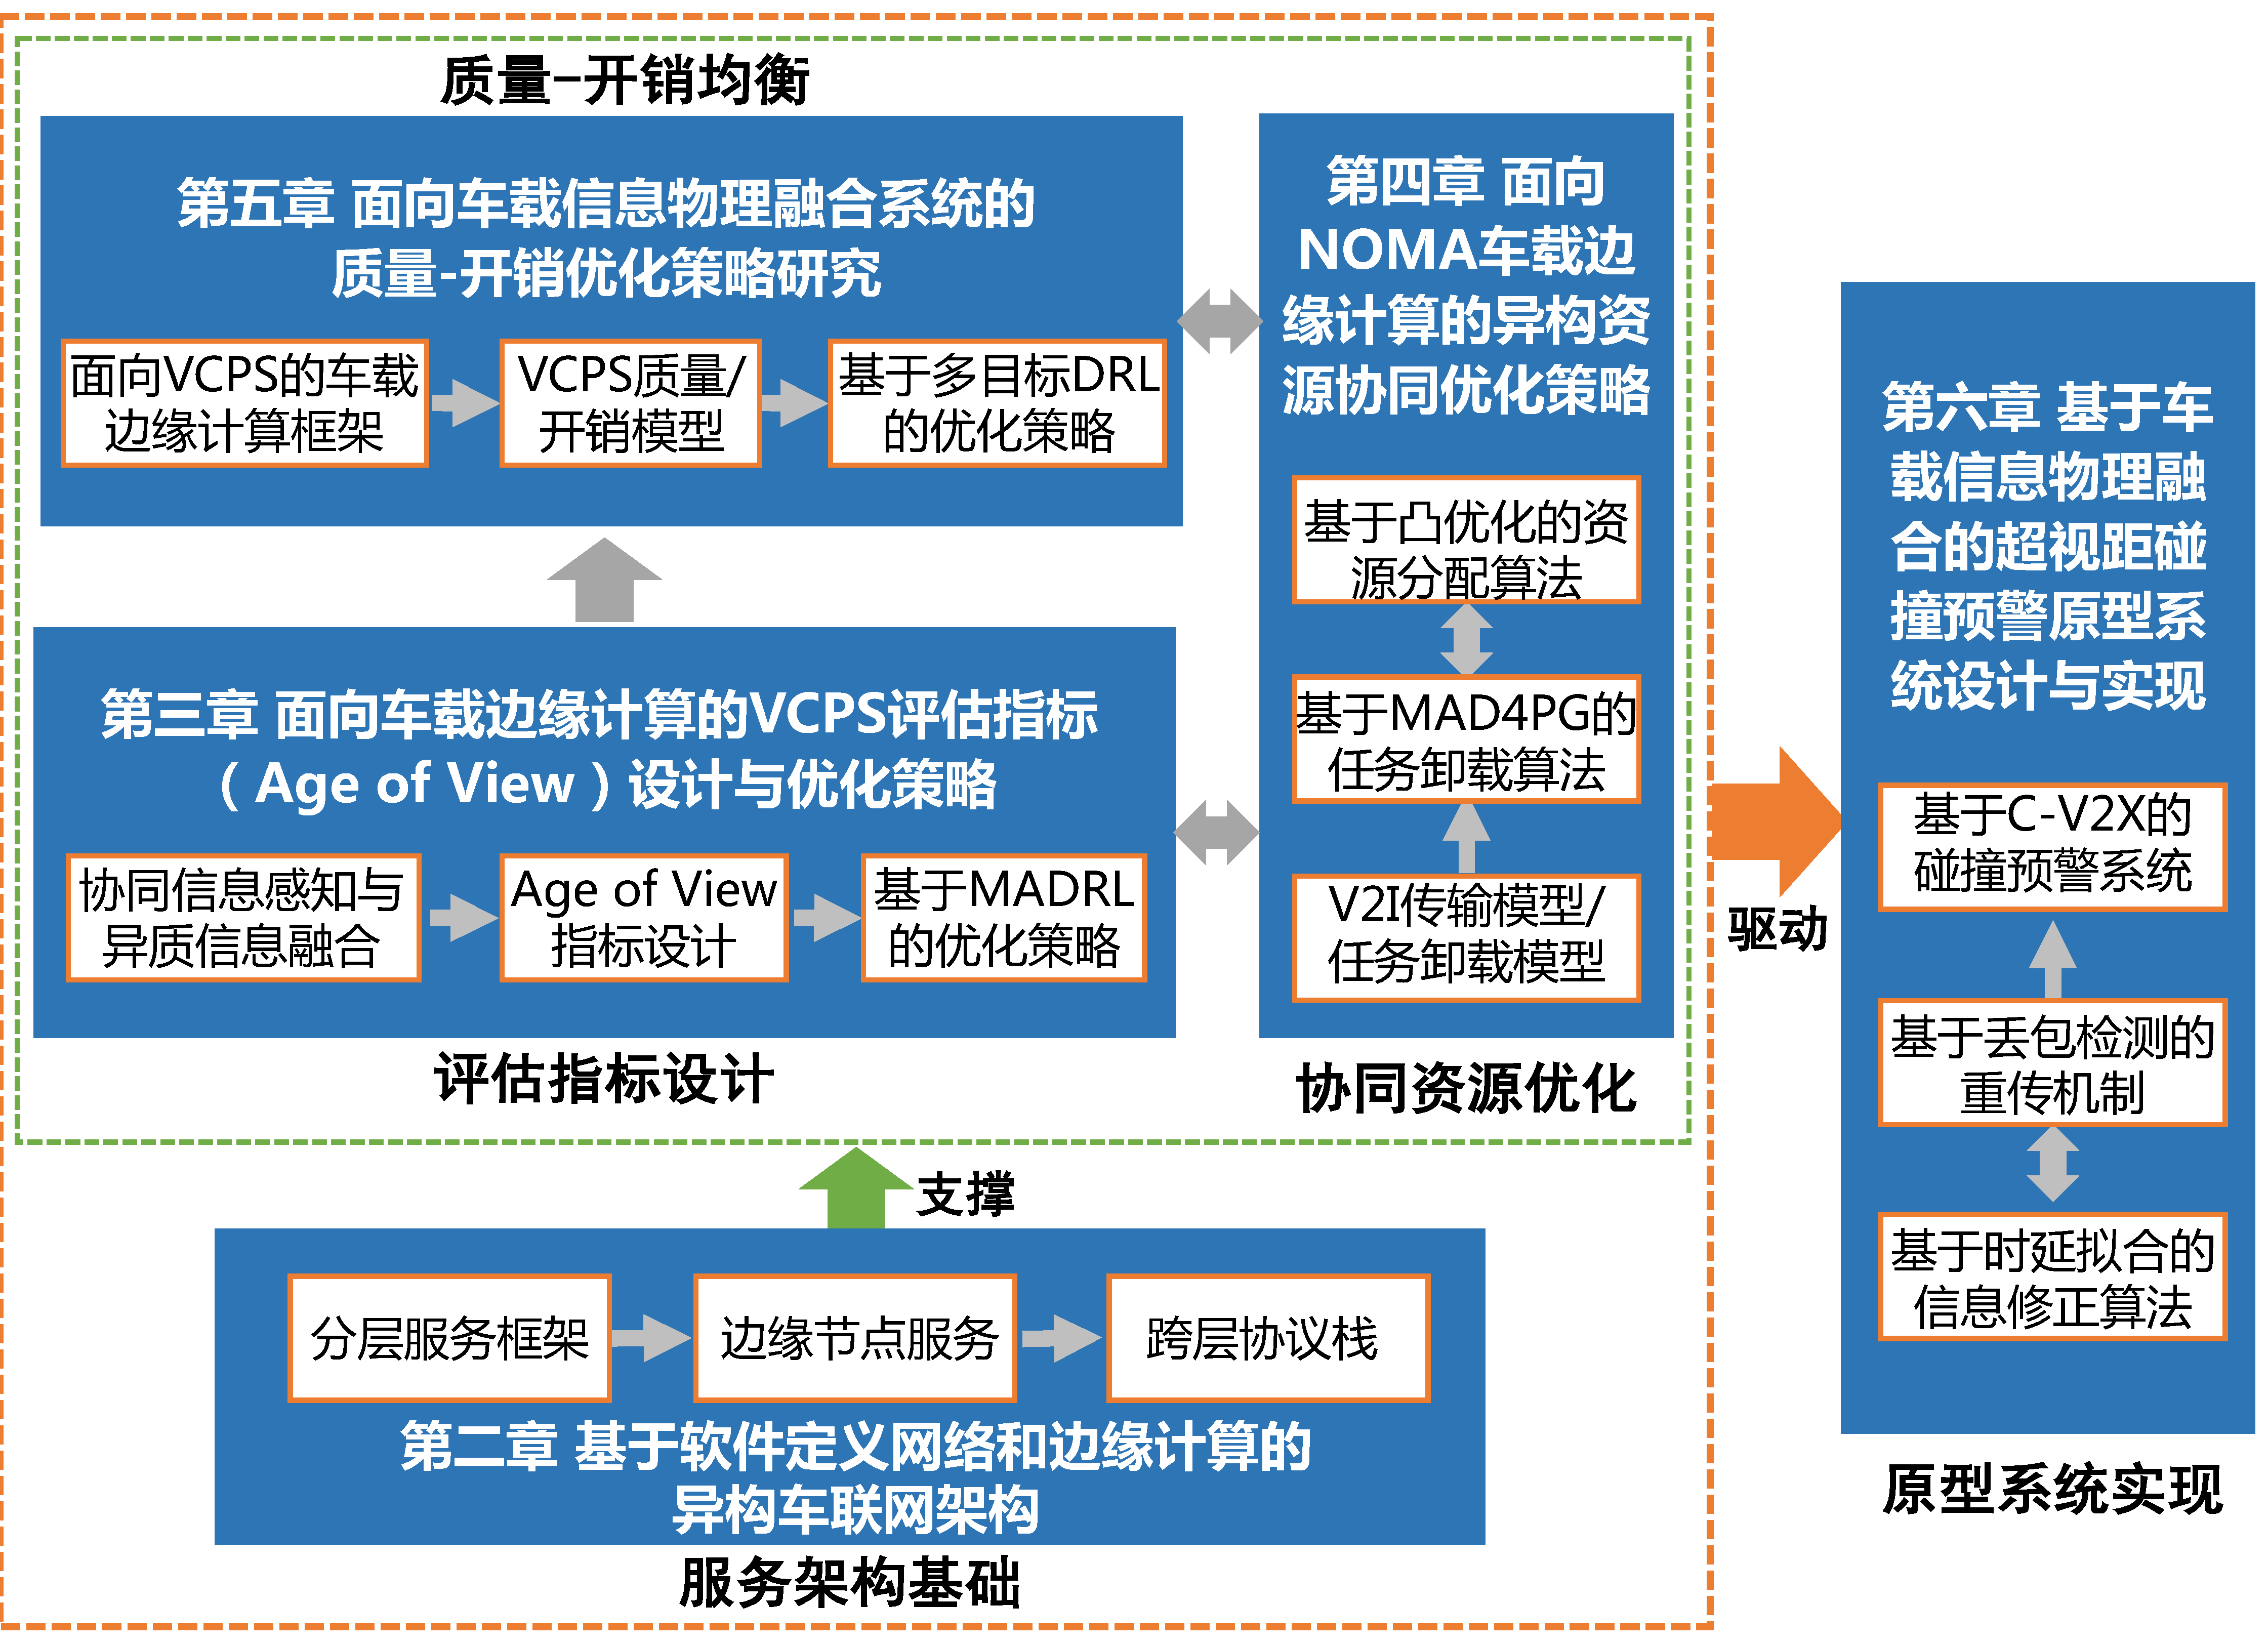
\includegraphics[width=1\columnwidth]{Fig1-2-content.pdf}
	\bicaption{主要研究内容}{Main research content}
	\label{fig 1-2}
\end{figure}

\circled{1} 基于软件定义网络和边缘计算的异构车联网架构研究

考虑车联网环境中的网络资源的高异构性、拓扑结构的高动态性,以及车辆节点的高移动性等关键特征,本文将以软件定义网络为基础,结合网络功能虚拟化、边缘计算与网络切片等关键思想,提出基于 SDN 和边缘计算的异构融合车联网新架构。本部分将重点研究基于 SDN 的异构网络分层服务架构、基于边缘计算的网络融合与分布式控制策略以及跨层协议栈。

\circled{2} 面向车载边缘计算的 VCPS 评估指标(Age of View)设计与优化策略研究

考虑车联网物理环境分布式时变性、感知信息维度与来源不同,以及车辆节点感知能力差异等关键特征,本文将针对物理信息的感知与建模进行研究,并提出车载信息物理融合系统评估指标与优化策略。本部分将重点研究车载边缘计算环境下车辆协同感知与边缘侧异质信息融合模型,进一步考虑信息的多维需求(时效性、完整性、一致性),设计边缘视图评估指标(Age of View)。在此基础上,研究基于多智能体强化学习的边缘视图优化策略。

\circled{3} 面向 NOMA 车载边缘计算的异构资源协同优化策略研究

考虑车联网高动态环境与高异构资源,本文将首先引入NOMA技术最大化利用车联网频谱资源,并提出基于边缘协同的异构资源优化策略。本部分将重点研究 V2I 传输与任务卸载模型,并在此基础上,研究基于博弈强化学习的异构资源协同优化策略,具体地,研究协同资源优化博弈模型并设计基于凸优化的资源分配算法与基于多智能体 D4PG 的任务卸载算法。

\circled{4} 面向车载信息物理融合系统的质量-开销均衡优化策略研究

考虑智慧交通系统中多元应用需求,本文将针对车联网中不同交通要素的数字孪生的质量与开销模型进行研究,并提出车载信息物理融合质量-开销均衡优化策略。本部分将重点研究面向 VCPS 的车载边缘计算框架,并综合考虑信息的多维需求与代价,研究车载信息物理融合质量-开销模型。在此基础上,深入研究基于多目标强化学习的车载信息物理融合质量-开销均衡优化策略。

\circled{5} 基于车载信息物理融合系统的超视距碰撞预警原型系统设计与实现

考虑复杂真实车联网环境,本文将建立基于真实车辆轨迹的综合仿真平台对所提出的服务架构、评估指标、优化策略与理论模型进行全方位的分析与评估。本文将基于 C-V2X 通信设备,在真实车联网环境中,研究基于时延拟合的信息修正算法与基于丢包检测的重传机制,并实现基于车载信息物理融合的超视距碰撞预警原型系统,进一步验证所提理论模型与优化策略。

\section{拟解决的关键问题}\label{section 1-5}

\subsection{问题阐述}

本文致力于从异构车联网服务架构、视图评估指标设计、异构资源协同优化、VCPS 质量-开销均衡,以及系统原型设计五个方面,协同驱动面向异构车联网的车载信息物理融合系统。
具体地,本文拟解决的关键问题包括:

\circled{1} 车联网异构网络融合

针对车联网高异构、高动态、高分布式等特征,在车联网中实现 SDN 的基本架构,建立异构车联网架构,是实现车载信息物理融合系统的架构基础。
在此基础上,进一步实现基于车载边缘计算的分布式服务策略,实现计算、存储、通信等物理资源的虚拟化与基于不同应用需求的动态资源分配与管理。
因此,如何实现基于 SDN 逻辑集中控制与基于边缘计算分布式控制与数据传输的有机结合,进一步完善异构车联网的体系架构,是本文首要解决的关键问题。

\circled{2} 边缘视图质量评估与构建

针对车联网中车辆感知任务具有分布范围广、信息维度高、时空依赖性强等特征,在车载边缘节点针对不同智慧交通系统应用需求实现视图质量的量化评估,是实现车载信息物理融合的数据支撑。
与此同时,车辆感知节点的移动性、感知能力差异性,进一步增加了在边缘节点融合物理信息、构建有效视图的难度。
因此,如何建立视图量化评估模型,并在此基础上从协同感知与异质信息融合两个层面研究有效的边缘视图构建机制,是本文亟待解决的关键问题。

\circled{3} 异构资源协同优化

针对车联网节点的异构异构能力、动态拓扑结构与通信连接的不确定性,在 NOMA 车载边缘计算环境中基于边缘协同实现异构资源协同优化,是实现车载信息物理融合系统的技术支持。
与此同时,车辆 V2I 通信中域间与域内干扰,以及车联网节点资源动态异构性进一步增加了协同任务卸载与资源调度的难度。
因此,如何针对车联网特征与节点资源特征实现异构资源协同优化,最大化资源利用效率,是本文亟待解决的另一关键问题。

\circled{4} VCPS 质量-开销均衡

针对多元智慧交通系统应用需求,车联网不同交通要素数字孪生的质量/开销需求,实现面向车载信息物理融合的质量-开销均衡,是实现车载信息物理融合的理论保障。
因此,如何针对不同智慧交通系统应用需求,基于车联网中不同要素数字孪生,建立相应的质量/开销模型,并进一步实现车载信息物理融合质量-开销均衡,是本文需要解决的又一关键问题。

\circled{5} 原型系统设计与实现

针对真实复杂车联网环境下验证所提理论模型及算法的需求,以及突出车载信息物理融合系统对于智慧交通系统应用支撑作用,设计并实现基于车载信息物理融合的超视距碰撞预警原型系统,是实现车载信息物理融合的系统验证。
因此,如何在真实复杂车联网环境下,利用实际 C-V2X 通信设备,实现基于车载信息物理融合的超视距碰撞预警系统,是本文最后解决的关键问题。

\subsection{技术路线}

本文技术路线如图 \ref{fig 1-3} 所示。首先,凝练关键科学问题:针对高动态异构车联网、分布式时变物理环境、动态异构节点资源、多元智慧交通系统应用需求,以及真实复杂车联网环境所带来的挑战,从异构车联网融合、视图评估指标设计、异构资源协同优化、质量-开销均衡,以及原型系统设计与实现五方面协同驱动面向异构车联网的车载信息物理融合系统。
在此基础上,制定本文研究内容:1)研究面向异构车联网的融合服务架构,实现基于 SDN 的逻辑集中控制与基于边缘计算的分布式服务有机结合,为实现车载信息物理融合提供服务架构基础。2)研究车载边缘计算环境下协同信息感知与边缘视图构建,设计边缘视图评估指标,为实现车载信息物理融合系统提供数据支撑。3)研究 NOMA 车载边缘计算环境下异构资源协同优化策略,提高资源利用率,为实现车载信息物理融合提供技术支持。4)研究面向车载信息物理融合系统的质量-开销均衡优化策略,实现VCPS质量-开销均衡,为实现车载信息物理融合系统提供理论保障。5)研究基于车载信息物理融合的超视距碰撞预警系统原型,为实现车载信息物理融合系统提供系统原型。

\begin{figure}[h]
\centering
	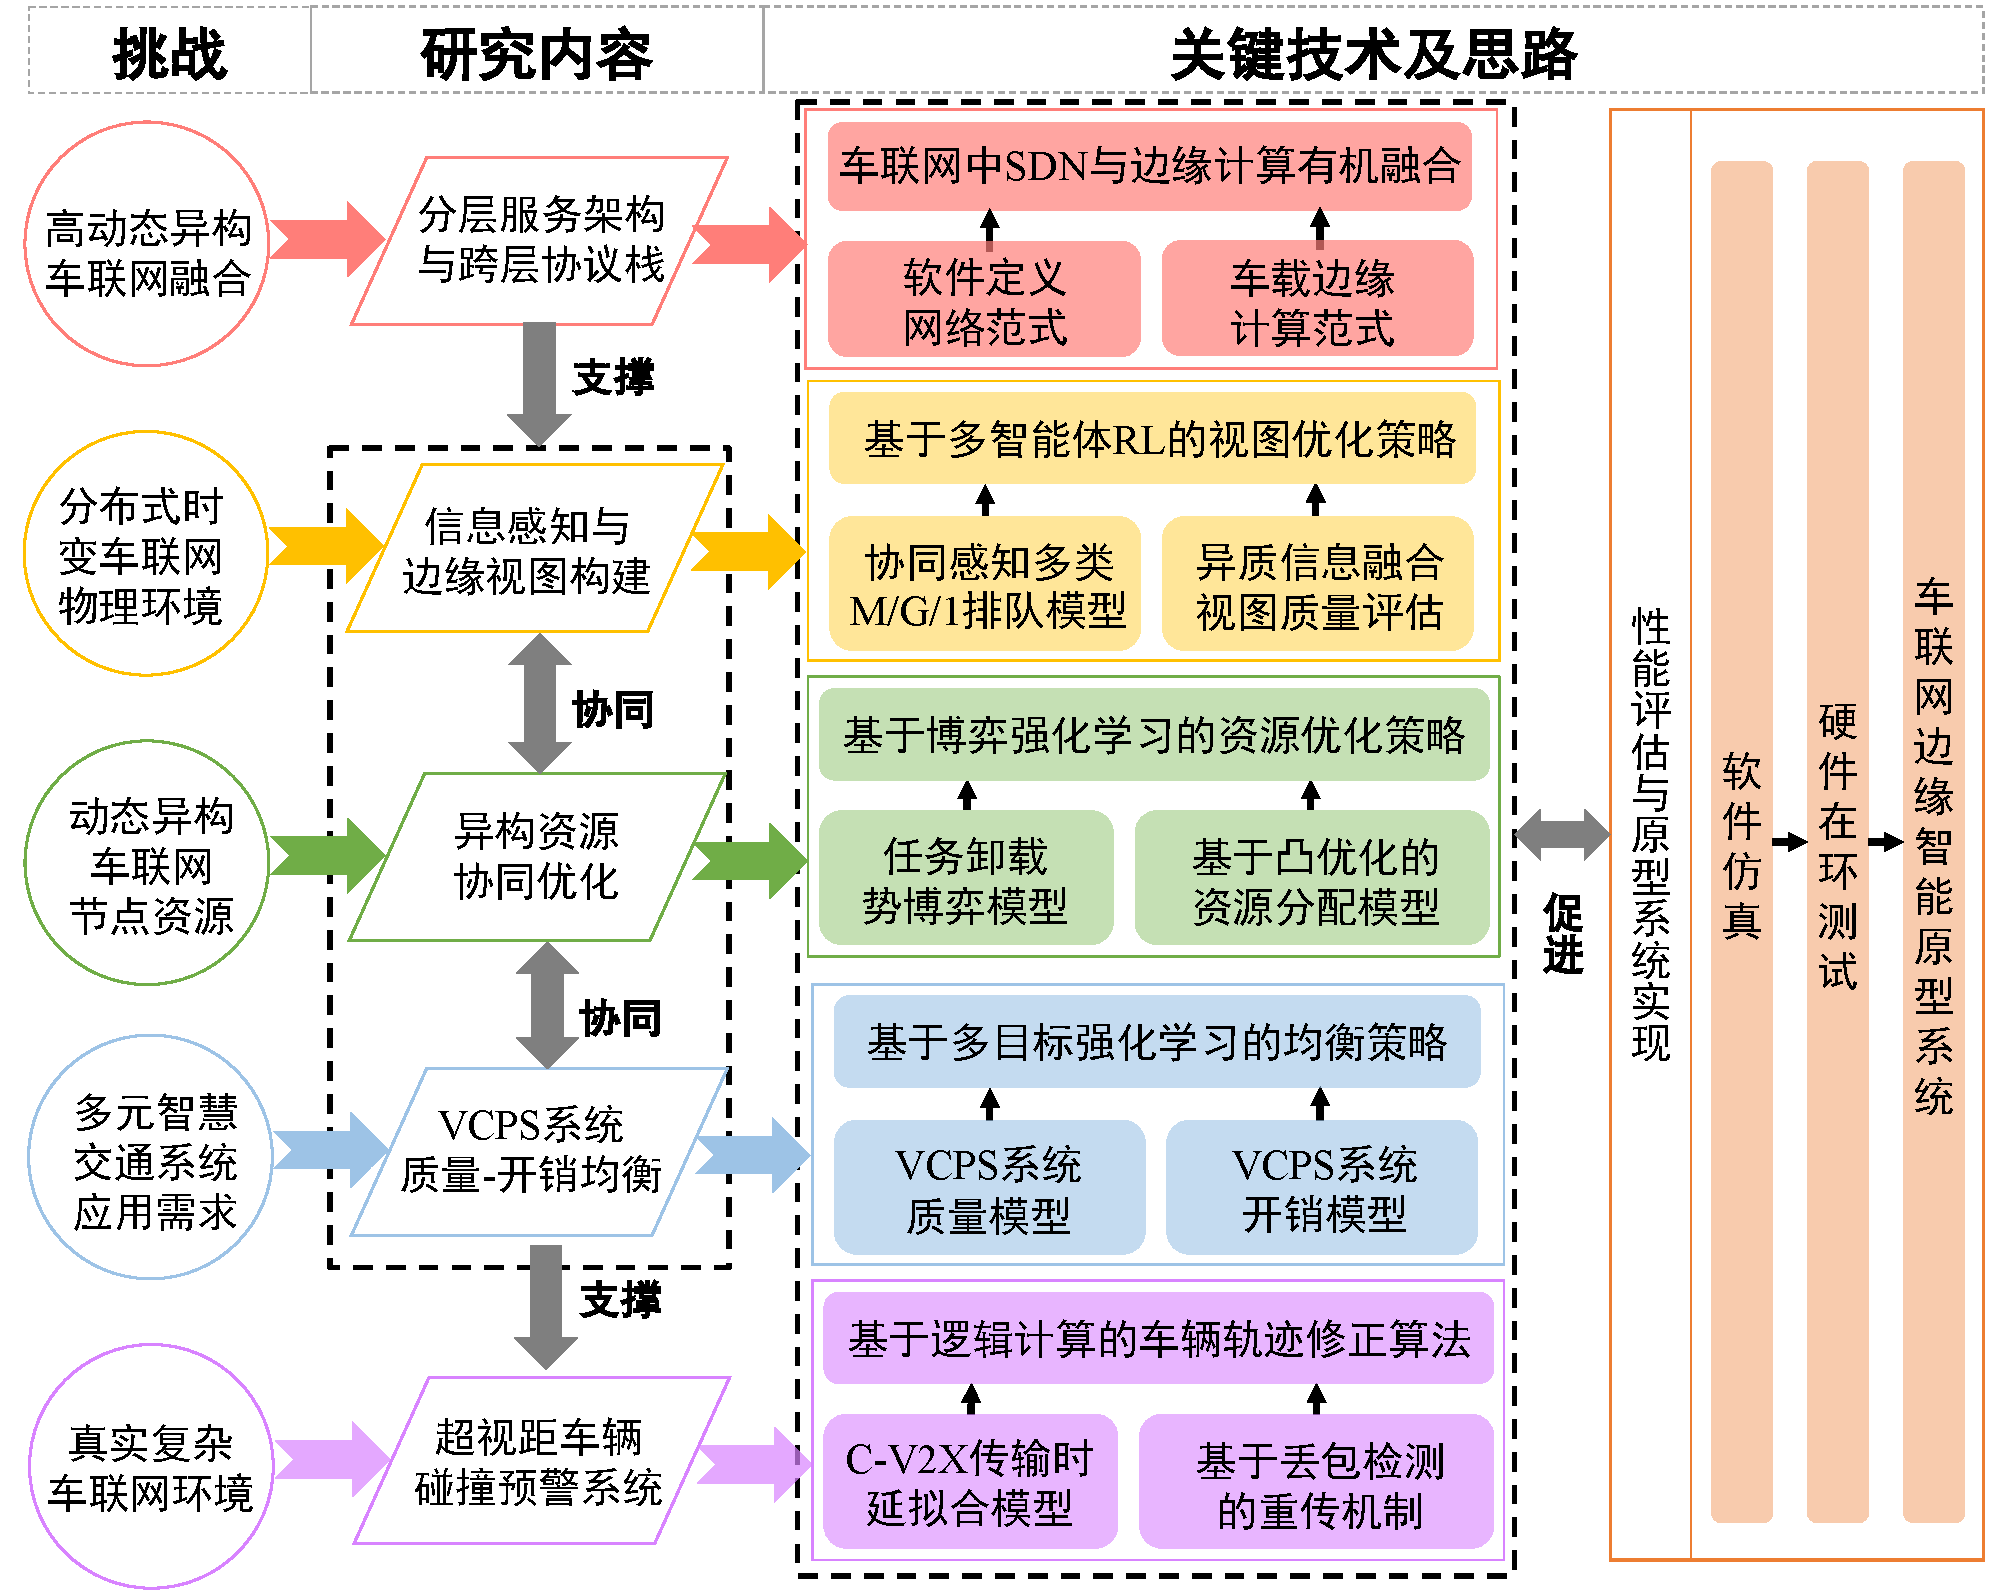
\includegraphics[width=1\columnwidth]{Fig1-3-technology-route.pdf}
	\bicaption{技术路线}{Technology route}
	\label{fig 1-3}
\end{figure}

最后,整理本文关键技术及思路:
1)针对研究内容1,首先提出基于软件定义网络的集中控制分层框架;其次,提出基于车载边缘计算的分布式服务策略与跨层协议栈;最后提出实现车联网中 SDN 与边缘计算有机融合的异构车联网服务架构。
2)针对研究内容2,首先提出基于多类 M/G/1 队列的协同感知模型;其次提出异质信息融合模型并设计边缘视图质量评估指标;最后提出基于多智能体强化学习的视图优化策略,实现边缘视图构建。
3)针对研究内容3,首先建立面向任务卸载的势博弈模型;其次,基于凸优化理论,提出通信资源分配模型;最后基于博弈强化学习,将任务卸载博弈转变为利用基于多智能体 D4PG 算法进行求解,实现异构资源协同优化。
4)针对研究内容4,首先针对多元智慧交通系统应用需求,提出 VCPS 质量模型与开销模型;最后基于多目标强化学习,设计 VCPS 质量-开销均衡优化策略。
5)针对研究内容5,首先提出基于C-V2X的无线传输时延拟合模型;其次提出基于丢包检测的重传机制;最后基于车载信息物理融合,设计基于逻辑计算的车辆轨迹修正算法,实现超视距碰撞预警系统原型。
6)搭建软件仿真环境、硬件在环测试平台,验证所提模型、机制与算法的可行性与有效性。在此基础上,针对具体应用场景,搭建系统原型,实现理论与应用相互促进。

\section{论文的特色与创新之处}\label{section 1-6}

本文致力于从服务架构、数据建模、资源调度、系统优化,以及原型实现五个层面协同研究并提炼面向异构车联网的车载信息物理融合关键科学问题,重点突破以下技术瓶颈:异构车联网融合、边缘视图评估与优化、异构资源协同优化、VCPS质量-开销均衡优化,以及原型系统设计与实现。
特别地,区别于现有单纯针对车联网的通信协议、服务架构、资源分配与智能应用等研究,本文从驱动面向异构车联网的车载信息物理融合系统的实际需求出发,分析当前面临的挑战,并针对车载信息物理融合系统的架构基础、数据支撑、技术支持、理论保障与原型系统五个方面提出关键问题。
本文具体特色体现在:
a)面对高异构、高动态、高分布式车联网环境,考虑车联网环境中的异构无线通信与移动数据节点所带来的挑战,研究如何将基于SDN的集中控制与基于边缘计算的分布式调度有机结合,为车载信息物理融合系统提供架构基础;
b)面向信息感知的时效性与准确性需求,考虑感知信息时变性、车辆节点移动性与感知能力差异性所带来的挑战,研究如何在车载边缘侧建立有效的物理信息视图,为车载信息物理融合系统提供数据支撑;
c)面向具有域内与域内干扰的 NOMA 车载边缘计算环境,考虑不同节点资源的动态异构性所带来的挑战,研究如何实现边缘协同最大化异构资源利用效率,为车载信息物理融合系统提供技术支持;
d)面向多元智慧交通系统应用需求,考虑车联网中不同交通要素数字孪生质量/开销需求差异带来的挑战,研究如何实现车载信息物理融合系统质量-开销均衡,为车载信息物理融合系统提供理论保障;
e)面向真实复杂车联网环境,考虑基于真实 C-V2X 通信设备部署与实现原型系统所带来的挑战,研究基于车载信息物理融合的超视距碰撞预警系统原型设计与实现,为车载信息物理融合系统提供原型系统。
本文主要创新点概括如下:

\circled{1} 提出综合 SDN、NFV、边缘计算与网络切片关键思想的异构融合车联网服务架构:现有车联网服务架构相关研究主要关注于单一范式的实践应用,同时,大多研究也为给出其中具体实现细节与深度思考,难以适用于具有大规模数据服务需求的下一代车联网场景与支撑车载信息物理融合系统。基于此,本文首先综合考虑高移动数据节点、高动态网络拓扑、高异构通信资源、高分布式系统环境等车联网特征,设计基于 SDN 集中控制与基于边缘计算分布式服务有机结合的异构车联网架构,并提出跨层协议栈,实现异构车联网有机融合。

\circled{2} 定义边缘视图概念,设计视图评估指标并建立视图质量评估模型,提出分布式协同信息感知与异质信息融合的边缘视图构建机制:现有研究重点关注于针对单一类型的时态数据建模与调度,难以面向异构车联网的车载信息物理融合系统形成有效的数据支撑。基于此,本文首先综合考虑感知信息特征(维度、时效性、关联性等)、感知任务属性(范围、周期、精度等)与感知节点属性(位置分布、通信连接、感知能力等),定义车联网边缘视图概念,建立针对视图质量的量化评估模型,并提出基于多智能体强化学习的边缘视图优化策略,实现车载边缘计算环境下的有效信息物理融合。

\circled{3} 提出基于边缘协同的通信/计算资源协同优化策略,打破传统针对单一资源的优化模式:现有面向车联网资源优化策略的研究主要集中于单一资源(通信、计算)的优化,难以满足不同任务对于车联网节点异构资源的需求。基于此,本文首先针对协同资源优化问题进行分解,将其转化为任务卸载与通信资源分配两个子问题。进一步,将任务卸载子问题建模为势博弈模型,并证明其具有纳什均衡与收敛性。最后,一方面,针对任务卸载博弈,基于多智能体 D4PG 算法提出任务卸载策略,另一方面,针对通信资源分配,基于凸优化提出通信资源分配策略。

\circled{4} 定义车载信息物理融合系统质量与开销模型,提出基于多目标强化学习的优化策略,注重于实现 VCPS 质量最大化的同时,满足 VCPS 开销最小:现有研究主要关注于基于车载信息物理融合系统的应用,忽略了车载信息物理融合过程中构建质量与开销。基于此,本文首先面向多元智慧交通系统应用的差异性需求,针对车联网中不同要素建立数字孪生模型。进一步,提出面向车联网中不同实体要素数字孪生的质量/开销模型。最后,基于多目标强化学习提出车载信息物理融合系统质量-开销均衡优化策略,实现VCPS质量-开销均衡。

\circled{5} 实现基于车载信息物理融合的超视距碰撞预警原型系统,在真实车联网环境下验证所提理论模型与优化策略:现有研究主要关注于基于仿真平台的实验验证,难以满足基于车载信息物理融合的实际 ITS 应用在真实车联网环境下的验证需求。基于此,本文首先建立基于C-V2X的无线传输时延拟合模型。进一步,提出基于丢包检测的重传机制。最后基于车载信息物理融合,设计基于逻辑计算的车辆轨迹修正算法,实现超视距碰撞预警系统原型。

综上,本文是建立在充分了解国内外相关领域学科前沿、清晰认识亟待解决的关键问题、合理制定研究目标与内容的基础上,是一项紧跟国际前沿的创新研究课题,是一项面向突破技术瓶颈、解决科学问题的基础研究课题,是一项理论结合实际的交叉研究课题。
本研究工作以车联网的特征和智慧交通系统应用需求为出发点,以车载信息物理融合为对象,以实现异构车联网中车载信息物理融合系统为目标,凝练出异构车联网融合、边缘视图评估与构建、异构资源协同优化、车载信息物理融合质量-开销均衡,以及原型系统设计与实现五方面的关键问题,并针对服务架构、评估指标设计、优化策略和系统原型进行深入研究,提出了面向异构车联网的车载信息物理融合的新架构、新指标、新模型、新理论和新算法,致力于实现车载信息物理融合系统,以支持多元智慧交通系统。
本文研究成果有助于完善车载信息物理融合理论体系,有助于推动智能网联汽车及相关应用的技术研发与标准制定,是有研究特色、有理论意义、有实用价值的。

\section{论文的组织结构}\label{section 1-7}
本文围绕异构车联网中车载信息物理融合系统相关问题展开了研究。具体来说,本文将结合车联网特征、智慧交通系统多元需求,从车联网的服务架构、评估指标设计、优化策略、原型系统实现方面进行理论与技术进行研究与创新,本文共分为7章节,详细内容如下。

第一章,绪论。首先,介绍了车载信息物理融合系统的研究背景和国内外相关研究现状。其次,阐述了本文的研究目标与详细内容。最后,总结了本文的组织结构。

第二章,基于软件定义网络和边缘计算的异构车联网架构研究。首先,提出了基于软件定义网络的分层服务架构,并介绍了网络功能虚拟化和网络切片,以及基于边缘计算的车联网服务。其次,详细阐述了控制层、虚拟化层、数据层面临的挑战,并设计了跨层协议栈。最后,通过真实场景中的案例研究对应用层的无线传输时延进行了拟合与分析,并给出了相应的启示。

第三章,面向车载边缘计算的VCPS评估指标(Age of View)设计与优化策略研究。首先,提出了面向车载信息物理融合系统的协同信息感知与异质信息融合框架。在此基础上,考虑到多元信息的时效性、一致性与完整性,设计了VCPS评估指标(Age of View,AoV), 并形式化定义了在车载边缘计算环境下最大化AoV问题。然后,提出了基于多智能体强化学习的调度算法。最后,构建了实验仿真模型并验证了所提指标与算法的优越性。

第四章,面向NOMA车载边缘计算的异构资源协同优化策略研究。首先,提出了面向NOMA车联网的车载边缘计算架构。其次,建立了V2I传输模型和任务卸载模型,在此基础上,形式化定义了协同资源优化问题。再次,将原问题建模为具有纳什均衡的势博弈模型,并设计了基于MAD4PG的任务卸载算法和基于凸优化的资源分配算法。最后,建立了实验评估模型并验证了所提算法的优越性。

第五章,面向车载信息物理融合系统的质量-开销优化策略研究。首先,提出了面向车联网数字孪生的车载边缘计算架构。其次,建立了协同感知模型和V2I上传模型,在此基础上,形式化定义了VCPS系统质量和系统开销,并给出了最大化系统质量与最小化系统开销的双目标问题。再次,提出了基于多目标强化学习的优化算法。最后,构建了实验仿真模型并验证了所提算法的优越性。

第六章,基于车载信息物理融合的超视距碰撞预警原型系统设计与实现研究。首先,建立了基于C-V2X的无线传输时延拟合模型。其次,提出了基于丢包检测的重传机制。最后,基于车载信息物理融合,设计了基于逻辑计算的车辆轨迹修正算法,实现超视距碰撞预警系统原型。

第七章,总结和展望。总结了全文研究的内容和贡献,并讨论了未来的研究方向与计划。






